
\chapter{逻辑}
\label{chap:logic}
\def\BKC{\cellcolor{gray!50}}   % cell background color

\section{排除法}
\begin{example}
  警察在审问四个嫌疑犯:甲,乙,丙,丁。他们的回话如下:
  \fbox{\parbox{\textwidth}{
      \begin{itemize}
      \item 甲说:我不是罪犯
      \item 乙说:丁是罪犯
      \item 丙说:乙是罪犯
      \item 丁说:我不是罪犯
      \end{itemize}
    }}
  研究完其它材料后警察发现以上四人只有一个人说假话。警察已经知道说假话的是罪犯,说真话的不是罪犯。那么,谁是罪犯?
\end{example}
\begin{proof}[提示]
  如果注意到乙和丁的话是互斥的,就会知道乙和丁中必有一人说的假话。从而甲和丙说的是真话,从而由丙的话可知乙说的是假话是罪犯。
  
  如果注意不到乙和丁的话是互斥的这一点,那么可以用通用的方法来找出说假话的人,即甲乙丙丁四人逐一排除,若剩余一人无法排除,则就是此人说假话。
  \begin{enumerate}
  \item 假设甲说假话,则其余三人说的都是真话,即以下四句为真:
    \begin{align*}
      \text{\numcircled1 甲是罪犯;\numcircled2 丁是罪犯;\numcircled3 乙是罪犯;\numcircled4 丁不是罪犯}
    \end{align*}
    从而有以下表格:

    \begin{center}
      \begin{tabular}{c|c|c|c|c}
        \hline
             & 甲 & 乙 & 丙 & 丁\\
        \hline
        罪犯 & $\checkmark^1$  & $\checkmark^3$  &    & $\checkmark^2\ \xmark^4$\\
        \hline
      \end{tabular}
    \end{center}

    其中\checkmark 代表此人是罪犯,$\xmark$代表此人不是罪犯,数字代表该符号对应于第几句话。由表格,可以看出两个矛盾的地方:\numcircled1 共有3个罪犯,但实际应只有一个罪犯;\numcircled2 丁既是罪犯又不是罪犯(既有\checkmark 符号,又有$\xmark$符号)。
    
    从而排除甲说假话。

  \item 假设乙说的假话,则其余三人说的是真话,即以下四句为真:
    \begin{align*}
      \text{\numcircled1 甲不是罪犯;\numcircled2 丁不是罪犯;\numcircled3 乙是罪犯;\numcircled4 丁不是罪犯}
    \end{align*}
    从而有以下表格:
    \begin{center}
      \begin{tabular}{c|c|c|c|c}
        \hline
             & 甲 & 乙 & 丙 & 丁\\
        \hline
        罪犯 & $\xmark^1$  & $\checkmark^3$  &    & $\xmark^2\ \xmark^4$\\
        \hline
      \end{tabular}
    \end{center}

    找不到矛盾。

  \item 假设丙说的是假话,则欺其余三人说的是真话,即以下四句为真:
    \begin{align*}
      \text{\numcircled1 甲不是罪犯;\numcircled2 丁是罪犯;\numcircled3 乙不是罪犯;\numcircled4 丁不是罪犯}
    \end{align*}
    从而有以下表格:

    \begin{center}
      \begin{tabular}{c|c|c|c|c}
        \hline
             & 甲 & 乙 & 丙 & 丁\\
        \hline
        罪犯 & $\xmark^1$  & $\xmark^3$  &    & $\checkmark^2\ \xmark^4$\\
        \hline
      \end{tabular}
    \end{center}
    从表格可以看出丁既是罪犯又不是罪犯,矛盾。排除丙说假话。
    
  \item 假设丁说的是假话,则欺其余三人说的是真话,即以下四句为真:
    \begin{align*}
      \text{\numcircled1 甲不是罪犯;\numcircled2 丁是罪犯;\numcircled3 乙是罪犯;\numcircled4 丁是罪犯}
    \end{align*}
    从而有以下表格:

    \begin{center}
      \begin{tabular}{c|c|c|c|c}
        \hline
             & 甲 & 乙 & 丙 & 丁\\
        \hline
        罪犯 & $\xmark^1$  & $\checkmark^3$  &    & $\checkmark^2\ \checkmark^4$\\
        \hline
      \end{tabular}
    \end{center}

    此处隐藏的条件是,说假话的是罪犯,说真话的不是罪犯。由于只有一个人说假话,从而只有一个罪犯,而由上面的表格容易看出乙和丁都是罪犯,这与只有一个罪犯矛盾。排除丁说假话。
  \end{enumerate}

  这样排除完甲丙丁三人,剩余一人,乙就是说假话的人,即罪犯就是乙。
\end{proof}


\begin{example}[歌唱家的年龄]
  甲乙丙丁四人正在讨论某位歌唱家的年龄:
  \begin{itemize}
  \item 甲说:她不会超过25岁。
  \item 乙说:她不会超过30岁。
  \item 丙说:她绝对在35岁以上。
  \item 丁说:她在40岁以下。
  \end{itemize}
  事实是这四人中只有一人说对了。那么请猜测下歌唱家的年龄范围。
\end{example}
\begin{proof}[提示]
  记歌唱家的真实年龄是$x$,那么四人的话等价于
  \begin{align*}
    \text{\numcircled1} x\le25,\quad \text{\numcircled2} x\le30,\quad \text{\numcircled3} x>35,\quad \text{\numcircled4} x<40
  \end{align*}
  如果用数轴表示,则会非常直观。

  \begin{center}
    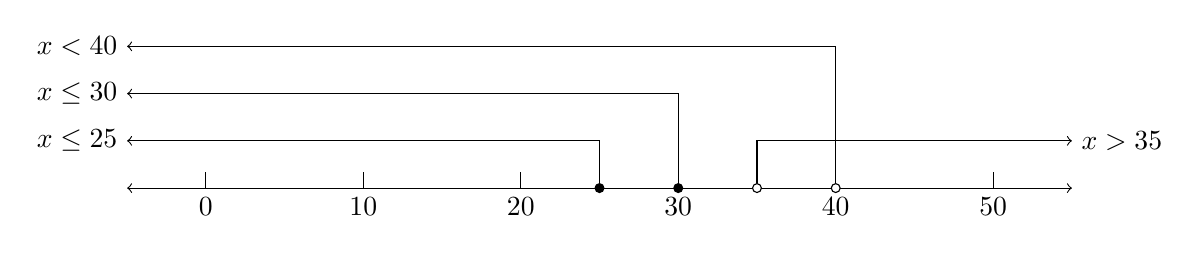
\begin{tikzpicture}[scale=.2]
      \draw[<->](-5,0)--(55,0);
      \foreach \x in {0,10,20,30,40,50}{
        \draw(\x,0) node[below]{$\x$}--(\x,1);
      }
      \draw[->](25,0)--(25,3)--(-5,3)node[left]{$x\le25$};
      \draw[->](30,0)--(30,6)--(-5,6)node[left]{$x\le30$};
      \draw[->](35,0)--(35,3)--(55,3)node[right]{$x>35$};
      \draw[->](40,0)--(40,9)--(-5,9)node[left]{$x<40$};
      \draw[fill=black](25,0)circle(8pt) (30,0)circle(8pt);
      \draw[fill=white](40,0)circle(8pt) (35,0)circle(8pt);
    \end{tikzpicture}
  \end{center}
  或者下面这种表示方式:
  \begin{center}
    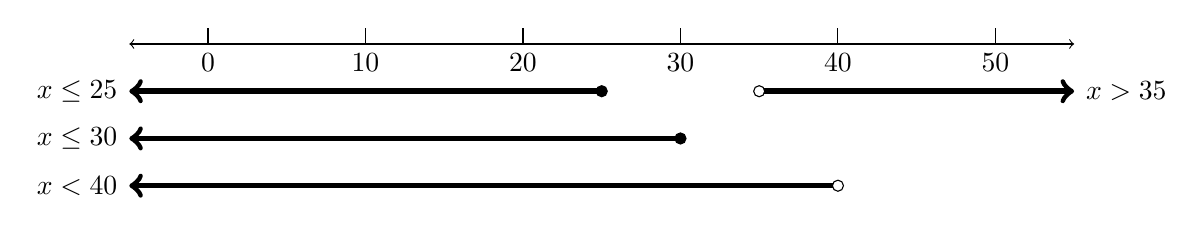
\begin{tikzpicture}[scale=.2]
      \draw[<->](-5,0)--(55,0);
      \foreach \x in {0,10,20,30,40,50}{
        \draw(\x,0) node[below]{$\x$}--(\x,1);
      }
      \draw[->,line width=2pt](25,-3)--(-5,-3)node[left]{$x\le25$};
      \draw[->,line width=2pt](30,-6)--(-5,-6)node[left]{$x\le30$};
      \draw[->,line width=2pt](35,-3)--(55,-3)node[right]{$x>35$};
      \draw[->,line width=2pt](40,-9)--(-5,-9)node[left]{$x<40$};
      \draw[fill=black](25,-3)circle(10pt) (30,-6)circle(10pt);
      \draw[fill=white](40,-9)circle(10pt) (35,-3)circle(10pt);
    \end{tikzpicture}
  \end{center}

  其中实心圈表示包含该点,空心圈表示不含此点。由上两图可以看出,只有$(30,35]$及$[40,+\infty)$这两个区间才是只被一个条件所覆盖的。
\end{proof}


\begin{example}
  有个遭遇到海难的人最终在一个小岛上顽强地生存了下来。有一天他被毒蛇咬伤了,需要用$3$升的纯净水来配药解毒,一点不能多一点不能少。但由于物资匮乏,他手里只有一个$5$升和$6$升的两个容器,以及之前他用蒸馏的方法获取到的足够多的备用纯净水。由于时间紧迫,请帮他用最少的步骤量出精确的$3$升纯净水。
\end{example}
\begin{proof}[提示]
  其中一种方法如表格~\ref{tab:water-ops}所示。经过若干步骤后6升容器里有纯净水3升。
  \begin{table}[htbp]
    \centering
    \caption{倒水操作}
    \label{tab:water-ops}
    \renewcommand*{\arraystretch}{1.0}
    \begin{tabular}{clcc}
      \toprule[1.5pt]
      % Use multicolumn to make the multirow center horizontally
      \multirow{2}{*}{步骤} & \multicolumn{1}{c}{\multirow{2}{*}{操作}} & \multicolumn{2}{c}{操作后容器含水量(升)} \\
      \cline{3-4}
           &      & $5$升容器 & $6$升容器 \\
      \midrule[1pt]
      0 & (开始状态)                       & 0 & 0\\
      \midrule[1pt]
      1 & 用备用纯净水灌满6升容器          & 0 & 6\\
      2 & 用6升容器里的水灌满5升容器       & 5 & 1\\
      3 & 清空5升容器                      & 0 & 1\\
      4 & 6升容器里的剩余的水全倒入5升容器 & 1 & 0\\
      5 & 用备用纯净水灌满6升容器          & 1 & 6\\
      6 & 用6升容器里的水灌满5升容器       & 5 & 2\\
      7 & 清空5升容器                      & 0 & 2\\
      8 & 6升容器里的剩余的水全倒入5升容器 & 2 & 0\\
      9 & 用备用纯净水灌满6升容器          & 2 & 6\\
     10 & 用6升容器里的水灌满5升容器       & 5 & 3\\
      \bottomrule[1.5pt]
    \end{tabular}
  \end{table}

  也可以用有向图的方法。记$(x,y)$分别为5升容器和6升容器中装了多少升水,则开始状态为$(0,0)$,目标状态为$(x,3)$或者$(3,y)$。
  \begin{center}\tiny
    \begin{tikzpicture}[scale=1.3]
      \node(N00)[draw,circle,pattern=north west lines,pattern color=blue!50]at(2,0){$0,0$};
      \node(N56)[draw,circle]at(1,0){$5,6$};

      \node(N50)[draw,circle]at(1,-1){$5,0$};
      \node(N05)[draw,circle]at(2,-1){$0,5$};
      \node(N55)[draw,circle]at(3,-1){$5,5$};
      \node(N46)[draw,circle]at(4,-1){$4,6$};
      \node(N40)[draw,circle]at(5,-1){$4,0$};
      \node(N04)[draw,circle]at(6,-1){$0,4$};
      \node(N54)[draw,circle]at(7,-1){$5,4$};
      \node(N36)[draw,circle,fill=red!50]at(8,-1){$3,6$};

      \node(N06)[draw,circle]at(1,1){$0,6$};
      \node(N51)[draw,circle]at(2,1){$5,1$};
      \node(N01)[draw,circle]at(3,1){$0,1$};
      \node(N10)[draw,circle]at(4,1){$1,0$};
      \node(N16)[draw,circle]at(5,1){$1,6$};
      \node(N52)[draw,circle]at(6,1){$5,2$};
      \node(N02)[draw,circle]at(7,1){$0,2$};
      \node(N20)[draw,circle]at(8,1){$2,0$};
      \node(N26)[draw,circle]at(9,1){$2,6$};
      \node(N53)[draw,circle,fill=red!50]at(10,1){$5,3$};

      \foreach \x/\y in{N00/N50,%
        N00/N06,N06/N51,N51/N01,N01/N10,N10/N16,N16/N52,N52/N02,N02/N20,N20/N26,N26/N53,%
        N05/N00%
      }{
        \draw[->](\x)--(\y);
      }
      \foreach \x/\y in{N06/N56,N50/N56,N50/N05,N05/N55,N55/N46,N46/N40,N40/N04,N04/N54,N54/N36}{
        \draw[->](\x)edge[bend left=20](\y);
        \draw[->](\y)edge[bend left=20](\x);
      }
      \foreach \x in{N40,N04}{
        \draw[->](\x)edge[bend right=20](N00);
      }
      \draw[->](N54)edge[bend left=30](N55);
      \draw[->](N54)edge[bend left=40](N50);
    \end{tikzpicture}
  \end{center}

  上图中箭头方向表示可由一个状态经过一个操作后到达另一个状态。当然,图中的结点及有向箭头是不全的\footnote{比如结点$(5,1)$经过一个操作后,可以达到的结点还有$(5,0)$、$(6,1)$,及$(5,6)$。},但也足以给出两种可以量出3升水的操作路径。
\end{proof}

\begin{question}
  古时候有家酒馆的老板特别节省,他只购买了一个7两和一个11两的勺子给客人打酒。有个刁钻的客人想要为难老板,于是一连10天跑去酒馆打酒,第一天只打一两,第二天打二两,第三天打三两,$\cdots\cdots$,第十天打十两。如果你是酒馆的老板,你如何应对这个客人的要求?
\end{question}
\begin{proof}[提示]
  类似地,可不停试验。

  其实可以归结为$7x+11y=1$的整数解问题,其解法参考第~\ref{chap:diophantine-equation}章~\nameref{chap:diophantine-equation}。其一个特解是$x=-3$,$y=2$。所以2个11两的倒满7两3次,可剩1两。$7x+11y=k$问题类似,其中$k$是任意正整数。
\end{proof}


\begin{example}
  小毛是学校出名的机灵鬼,也是家里让人头疼的调皮蛋。有一天他急急忙忙写完作业就要出动玩,妈妈便说还有一道题,要做完了才能出去玩。妈妈的题目是这样的:有6个杯子排成一排,前面3个装满了水,后面3个是空的。若只能移动一个杯子,能否将装满水的水杯与空杯间隔开?
\end{example}
\begin{proof}[提示]
  若“移动”还包括倒水的动作,那么是有可能的。只需要将前三杯中间的杯子里的水倒到后三杯中间的空杯子里,然后再放回原位即可。
  \begin{center}
    \begin{tikzpicture}[scale=1.0]
      \foreach \x in {0,1,2,3,4,5}{
      \begin{scope}[shift={(2 * \x,0)}]
        \coordinate(A)at(0,1.2);
        \coordinate(B)at(0.2,0);
        \coordinate(C)at(0.6,0);
        \coordinate(D)at(0.8,1.2);
        \coordinate(W1)at(0.05,1);
        \coordinate(W2)at(0.1,1.1);
        \coordinate(W3)at(0.2,1);
        \coordinate(W4)at(0.3,1.1);
        \coordinate(W5)at(0.4,1);
        \coordinate(W6)at(0.5,1.1);
        \coordinate(W7)at(0.6,1);
        \coordinate(W8)at(0.7,1.1);
        \coordinate(W9)at(0.75,1);
        \ifthenelse{\x<3}{
          \fill[pattern=dots,pattern color=blue!30](W1)--(W2)--(W3)--(W4)--(W5)--(W6)--(W7)--(W8)--(W9)--(C)--(B)--cycle;
          \draw[color=blue!30](W1)--(W2)--(W3)--(W4)--(W5)--(W6)--(W7)--(W8)--(W9);
        }{}
        \draw(A)--(B)--(C)--(D);
      \end{scope}
      }
      \node(X)at(2.4,-.2){};
      \node(Y)at(8.4,-.2){};
      \draw[->](X) to[out=330,in=210](Y);
      \node at(5.4,-.7){倒水};
    \end{tikzpicture}
  \end{center}
  % don't show qed symbol for this example only
  \let\qed\relax
\end{proof}

\begin{example}[爱因斯坦难题]\label{ex:einstein's-problem}
  在一条街上,有5座房子,喷了5种颜色。每个房子了住着不同国籍的人,每个人
  喝着不同的饮料,抽不同品牌的香烟,养着不同的宠物,这有一些他们的信
  息:
  \begin{enumerate}
  \item 英国人住在红房子里,
  \item 瑞典人养了一条狗,
  \item 丹麦人喝茶,
  \item 绿房子在白房子左边(注:是指紧挨着的左边),
  \item 绿房子主人喝咖啡,
  \item 抽PALL MALL烟的人养了一只鸟,
  \item 黄房子主人抽DUNHILL烟,
  \item 住在中间那间房子的人喝牛奶,
  \item 挪威人住第一间房子,
  \item 抽BLENDS烟的人住在养猫人的旁边,
  \item 养马的人住在DUNHILL烟的人旁边,
  \item 抽BLUE MASTER烟的人喝啤酒,
  \item 德国人抽PRINCE烟,
  \item 挪威人住在蓝房子旁边,
  \item 抽BLENDS烟的人的邻居喝矿泉水。
  \end{enumerate}
  那么谁在养鱼?
\end{example}
\begin{proof}[提示]
  做表格,一个个排除,一个个填,与数独类似。

  首先由(8)和(9),可以先填入下表:
    \begin{center}
      \renewcommand*{\arraystretch}{1.0}
      \begin{tabular}{l|l|l|l|l|l}
        \hline
        房号     & 1      & 2 & 3    & 4 & 5\\\hline
        颜色     &        &   &      &   &  \\\hline
        国籍     & 挪威人 &   &      &   &  \\\hline
        饮料     &        &   & 牛奶 &   &  \\\hline
        烟       &        &   &      &   &  \\
        宠物     &        &   &      &   &  \\
        \hline
      \end{tabular}
    \end{center}

    再由(14),填入蓝房子
    \begin{center}
      \renewcommand*{\arraystretch}{1.0}
      \begin{tabular}{l|l|l|l|l|l}
        \hline
        房号     & 1      & 2  & 3    & 4 & 5\\\hline
        颜色     &        & 蓝 &      &   &  \\\hline
        国籍     & 挪威人 &    &      &   &  \\\hline
        饮料     &        &    & 牛奶 &   &  \\\hline
        烟       &        &    &      &   &  \\\hline
        宠物     &        &    &      &   &  \\
        \hline
      \end{tabular}
    \end{center}

    再由(1)和(4),红、绿、白房子只能都在3、4 、5号房子里,从而1号是黄房子。由(7)可填入1号房子主人抽什么。再由(11)可填入马。
    \begin{center}
      \renewcommand*{\arraystretch}{1.0}
      \begin{tabular}{l|l|l|l|l|l}
        \hline
        房号     & 1      & 2  & 3    & 4 & 5\\\hline
        颜色     & 黄     & 蓝 &      &   &  \\\hline
        国籍     & 挪威人 &    &      &   &  \\\hline
        饮料     &        &    & 牛奶 &   &  \\\hline
        烟       & DUNHILL&    &      &   &  \\\hline
        宠物     &        & 马 &      &   &  \\
        \hline
      \end{tabular}
    \end{center}

    再由(4),“绿白”要紧挨着填入,只能填“34”或“45”号房子。由(5),“绿”不能是3号房子,从而“绿白”要填入“45”号房子,继而3号房子是红房子,再由(1),填入英国人。由(5)填入咖啡。
    \begin{center}
      \renewcommand*{\arraystretch}{1.0}
      \begin{tabular}{l|l|l|l|l|l}
        \hline
        房号     & 1      & 2  & 3     & 4     & 5\\\hline
        颜色     & 黄     & 蓝 & 红    & 绿    &白\\\hline
        国籍     & 挪威人 &    & 英国人&       &  \\\hline
        饮料     &        &    & 牛奶  & 咖啡  &  \\\hline
        烟       & DUNHILL&    &       &       &  \\\hline
        宠物     &        & 马 &       &       &  \\
        \hline
      \end{tabular}
    \end{center}

    此时,划掉已经无用的条件,剩余如下:
    \begin{enumerate}
    \item \sout{英国人住在红房子里,}
    \item 瑞典人养了一条狗,
    \item 丹麦人喝茶,
    \item \sout{绿房子在白房子左边(注:是指紧挨着的左边),}
    \item \sout{绿房子主人喝咖啡,}
    \item 抽PALL MALL烟的人养了一只鸟,
    \item \sout{黄房子主人抽DUNHILL烟,}
    \item \sout{住在中间那间房子的人喝牛奶,}
    \item \sout{挪威人住第一间房子,}
    \item 抽BLENDS烟的人住在养猫人的旁边,
    \item \sout{养马的人住在DUNHILL烟的人旁边,}
    \item 抽BLUE MASTER烟的人喝啤酒,
    \item 德国人抽PRINCE烟,
    \item \sout{挪威人住在蓝房子旁边,}
    \item 抽BLENDS烟的人的邻居喝矿泉水。
    \end{enumerate}

    由(3),“丹麦人”和“喝茶”两个一起填入的只剩下2号和5号房。由(12),“抽BLUE MASTER”和“喝啤酒”两个一起填入的也只剩下2号和5号房。再由(15),还有人“喝矿泉水”。此时可知“喝矿泉水”的是1号房,并且2号房抽BLENDS烟。
    \begin{center}
      \renewcommand*{\arraystretch}{1.0}
      \begin{tabular}{l|l|l|l|l|l}
        \hline
        房号     & 1      & 2      & 3     & 4     & 5\\\hline
        颜色     & 黄     & 蓝     & 红    & 绿    &白\\\hline
        国籍     & 挪威人 &        & 英国人&       &  \\\hline
        饮料     & 矿泉水 &        & 牛奶  & 咖啡  &  \\\hline
        烟       & DUNHILL& BLENDS &       &       &  \\\hline
        宠物     &        & 马     &       &       &  \\
        \hline
      \end{tabular}
    \end{center}

    此时再由(12),能够一起填入抽BLUE MASTER和喝啤酒的就只剩下5号房了,从而可在5号房填入BLUE MASTER和啤酒。这样之后由(3),丹麦人和苶就只能填在2号房了。再划掉(3)、(12),表格及剩余条件如下。
    \begin{center}
      \renewcommand*{\arraystretch}{1.0}
      \begin{tabular}{l|l|l|l|l|l}
        \hline
        房号     & 1      & 2      & 3     & 4     & 5           \\\hline
        颜色     & 黄     & 蓝     & 红    & 绿    &白           \\\hline
        国籍     & 挪威人 & 丹麦人 & 英国人&       &             \\\hline
        饮料     & 矿泉水 & 茶     & 牛奶  & 咖啡  &啤酒         \\\hline
        烟       & DUNHILL& BLENDS &       &       &BLUE MASTER  \\\hline
        宠物     &        & 马     &       &       &  \\
        \hline
      \end{tabular}
    \end{center}

    \begin{enumerate}
    \item \sout{英国人住在红房子里,}
    \item 瑞典人养了一条狗,
    \item \sout{丹麦人喝茶,}
    \item \sout{绿房子在白房子左边(注:是指紧挨着的左边),}
    \item \sout{绿房子主人喝咖啡,}
    \item 抽PALL MALL烟的人养了一只鸟,
    \item \sout{黄房子主人抽DUNHILL烟,}
    \item \sout{住在中间那间房子的人喝牛奶,}
    \item \sout{挪威人住第一间房子,}
    \item 抽BLENDS烟的人住在养猫人的旁边,
    \item \sout{养马的人住在DUNHILL烟的人旁边,}
    \item \sout{抽BLUE MASTER烟的人喝啤酒,}
    \item 德国人抽PRINCE烟,
    \item \sout{挪威人住在蓝房子旁边,}
    \item 抽BLENDS烟的人的邻居喝矿泉水。
    \end{enumerate}

    此时由(13),德国人抽PRINCE烟只能在4号房。由(2),剩下的瑞典人养狗只能在5号房。由(6),PALL MALL烟和养鸟在3号房。
    \begin{center}
      \renewcommand*{\arraystretch}{1.0}
      \begin{tabular}{l|l|l|l|l|l}
        \hline
        房号     & 1      & 2      & 3         & 4     & 5           \\\hline
        颜色     & 黄     & 蓝     & 红        & 绿    &白           \\\hline
        国籍     & 挪威人 & 丹麦人 & 英国人    & 德国人&瑞典人       \\\hline
        饮料     & 矿泉水 & 茶     & 牛奶      & 咖啡  &啤酒         \\\hline
        烟       & DUNHILL& BLENDS & PALL MALL & PRINCE&BLUE MASTER  \\\hline
        宠物     &        & 马     & 鸟        &       &狗           \\
        \hline
      \end{tabular}
    \end{center}

    此时由(10),养猫只能在1号房。从而表格中只剩余4号房养什么宠物未知。而由题目是问谁养鱼,故养鱼只能填在4号房。
\end{proof}

\begin{example}
  六所房子排成一排,每所房子颜色不同,每位屋主来自不同的地方,吃着不同的水果,喝着不同的饮料,喜欢不同的运动,养不同的宠物。下面是关于他们的一些信息:\
  \begin{enumerate}%\vspace{-2cm}
  \begin{multicols}{2}
  \item 前3位无养鸡和吃葡萄者。
  \item 吃桔子的人也养马。
  \item 北京人在养鸟者旁边。
  \item 湖南人住黄房子。
  \item 四川人旁边的人吃桔子。
  \item 绿房子的主人吃西瓜。
  \item 上海人在白房子旁边。
  \item 江苏人喜欢打排球。
  \item 红色屋主喝牛奶。
  \item 养猫人在第一所房子。
  \item 打篮球的人养狗。
  \item 喝咖啡的人吃香蕉。
  \item 打棒球的人养鸡。
  \end{multicols}%\vspace{-2cm}
  \item 喝茶者在喝矿泉水者的右边
  \item 爱吃香蕉者和打棒球者住在中间(第3、4位置)
  \item 后3位中没有黑房子,有吃苹果者。
  \item 篮球、垒球、足球,这3项运动的爱好者互不相邻。
  \item 上海人和黑房子之间隔有3个位置。
  \item 白色房子既不在中间,也不在最后,与蓝房子相邻。
  \item 喝可乐者和山东人之间仅隔喝啤酒者。
  \item 爱吃苹果的人也爱打桌球。
  \item 吃桃子者与打桌球者之间仅隔扔垒球者。
  \end{enumerate}
那么谁养鱼?
\end{example}

\newcolumntype{Y}{>{\centering\arraybackslash}X}
\begin{center}
  %https://tex.stackexchange.com/questions/60601/evenly-distributing-column-widths
  
  \begin{tabularx}{\textwidth}{|c *{7}{|Y}}
    \hline
    房间 & 1 & 2 & 3 & 4 & 5 & 6\\\hline
    颜色 &   &   &   &   &   &  \\\hline
    地方 &   &   &   &   &   &  \\\hline
    水果 &   &   &   &   &   &  \\\hline
    饮料 &   &   &   &   &   &  \\\hline
    运动 &   &   &   &   &   &  \\\hline
    宠物 &   &   &   &   &   &  \\\hline
  \end{tabularx}
\end{center}

\noindent\begin{minipage}{\textwidth}\setlength{\parindent}{2em}
先根据(10),填猫。根据(1)、(13)和(15),填棒球、鸡和香蕉。再由(12)填入咖啡。
\begin{center}
  \begin{tabularx}{\textwidth}{|c *{7}{|Y}}
    \hline
    房间 & 1 & 2 & 3     & 4 & 5 & 6\\\hline
    颜色 &   &   &       &       &   &  \\\hline
    地方 &   &   &       &       &   &  \\\hline
    水果 &   &   & 香蕉  &       &   &  \\\hline
    饮料 &   &   & 咖啡  &       &   &  \\\hline
    运动 &   &   &       & 棒球  &   &  \\\hline
    宠物 & 猫&   &       & 鸡    &   &  \\\hline
  \end{tabularx}\vspace{.5cm}
\end{center}
\end{minipage}

\noindent\begin{minipage}{\textwidth}\setlength{\parindent}{2em}
由(21)和(22),苹果、桌球、桃子和垒球只能是以下两种排列方式:\nopagebreak
\begin{center}
  \begin{tabular}{|c|c|c|}
    \hline
    \BKC 苹果 & & \BKC 桃子\\\hline
    & & \\\hline
    \BKC 桌球 & \BKC 垒球 &\\\hline
  \end{tabular}
  \hspace{2cm}
  \begin{tabular}{|c|c|c|}
    \hline
    \BKC 桃子 & & \BKC 苹果\\\hline
    & & \\\hline
     & \BKC 垒球 & \BKC 桌球\\\hline
  \end{tabular}\vspace{.5cm}
\end{center}
\end{minipage}

\noindent\begin{minipage}{\textwidth}\setlength{\parindent}{2em}
再由(16)苹果在4/5/6号房,从而只有上面第二种排列能放入到表格中:\nopagebreak
\begin{center}
  \begin{tabularx}{\textwidth}{|c *{7}{|Y}}
    \hline
    房间 & 1 & 2 & 3     & 4    & 5    & 6   \\\hline
    颜色 &   &   &       &      &      &     \\\hline
    地方 &   &   &       &      &      &     \\\hline
    水果 &   &   & 香蕉  & \BKC 桃子  &      & \BKC 苹果 \\\hline
    饮料 &   &   & 咖啡  &      &      &     \\\hline
    运动 &   &   &       & 棒球  & \BKC 垒球 & \BKC 桌球 \\\hline
    宠物 & 猫&   &       & 鸡    &      &     \\\hline
  \end{tabularx}\vspace{.5cm}
\end{center}
\end{minipage}

\noindent\begin{minipage}{\textwidth}\setlength{\parindent}{2em}
由(17),足球、篮球占据了房间1和3。由(11),打篮球养狗的人只能在(3),从而足球在(1)。由(8),剩下打排球的江苏人在(2)。由(1),葡萄在(5)。\nopagebreak
\begin{center}
  \begin{tabularx}{\textwidth}{|c *{7}{|Y}}
    \hline
    房间 & 1   & 2 & 3     & 4    & 5    & 6   \\\hline
    颜色 &     &   &       &      &      &     \\\hline
    地方 &     & \BKC 江苏  &       &      &      &     \\\hline
    水果 &     &   & 香蕉  & 桃子  & \BKC 葡萄 & 苹果 \\\hline
    饮料 &     &   & 咖啡  &      &      &     \\\hline
    运动 & \BKC 足球 & \BKC 排球 & \BKC 篮球   & 棒球  & 垒球 & 桌球 \\\hline
    宠物 & 猫  &   & \BKC 狗    & 鸡    &      &     \\\hline
  \end{tabularx}\vspace{.5cm}
\end{center}
\end{minipage}

\noindent\begin{minipage}{\textwidth}\setlength{\parindent}{2em}
此时剩余1号房和2号房两种水果。由(5),桔子不能在1号房,从而桔子在2号房。由(6),填入绿色和西瓜。由(2),填入马。\nopagebreak
\begin{center}
  \begin{tabularx}{\textwidth}{|c *{7}{|Y}}
    \hline
    房间 & 1   & 2     & 3     & 4    & 5    & 6   \\\hline
    颜色 & \BKC 绿色 &      &       &      &      &     \\\hline
    地方 &     & 江苏  &       &      &      &     \\\hline
    水果 & \BKC 西瓜 & \BKC 桔子 & 香蕉  & 桃子  & 葡萄 & 苹果 \\\hline
    饮料 &     &     & 咖啡   &      &      &     \\\hline
    运动 & 足球 & 排球 & 篮球   & 棒球  & 垒球 & 桌球 \\\hline
    宠物 & 猫  & \BKC 马  & 狗    & 鸡    &      &     \\\hline
  \end{tabularx}\vspace{.5cm}
\end{center}
\end{minipage}

\noindent\begin{minipage}{\textwidth}\setlength{\parindent}{2em}
由(16),黑色在2号或3号,从而由(18),上海在6号或7号(不存在),从而黑色在2号,上海在6号。由(19),白色在5号。
\begin{center}
  \begin{tabularx}{\textwidth}{|c *{7}{|Y}}
    \hline
    房间 & 1   & 2     & 3    & 4    & 5    & 6   \\\hline
    颜色 & 绿色 & \BKC 黑色 &  & % \BKC 黄
    & \BKC 白色  &     \\\hline
    地方 &     & 江苏  &      & % \BKC 湖南
    &      & \BKC 上海 \\\hline
    水果 & 西瓜 & 桔子 & 香蕉  & 桃子  & 葡萄 & 苹果 \\\hline
    饮料 &     &      & 咖啡  &      &      &     \\\hline
    运动 & 足球 & 排球 & 篮球  & 棒球  & 垒球 & 桌球 \\\hline
    宠物 & 猫  &  马  & 狗    & 鸡    &      &     \\\hline
  \end{tabularx}\vspace{.5cm}
\end{center}
\end{minipage}

\noindent\begin{minipage}{\textwidth}\setlength{\parindent}{2em}
由(19),蓝色在4、6。由(9),红色在4、6。从而由(4),剩余的一个黄色在3,填入湖南与黄色。由(5),四川人在1号。
\begin{center}
  \begin{tabularx}{\textwidth}{|c *{7}{|Y}}
    \hline
    房间 & 1   & 2     & 3   & 4    & 5    & 6   \\\hline
    颜色 & 绿色 & 黑色 & \BKC 黄色 &    & 白色  &     \\\hline
    地方 & \BKC 四川 & 江苏  & \BKC 湖南 &     &      & 上海 \\\hline
    水果 & 西瓜 & 桔子 & 香蕉  & 桃子  & 葡萄 & 苹果 \\\hline
    饮料 &     &      & 咖啡  &      &      &     \\\hline
    运动 & 足球 & 排球 & 篮球  & 棒球  & 垒球 & 桌球 \\\hline
    宠物 & 猫  &  马  & 狗    & 鸡    &      &     \\\hline
  \end{tabularx}\vspace{.5cm}
\end{center}
\end{minipage}

\noindent\begin{minipage}{\textwidth}\setlength{\parindent}{2em}
由(20),山东、可乐、啤酒的排列形式只有以下两种:
\begin{center}
  \begin{tabular}{|c|c|c|}
    \hline
    \BKC 山东 &     &\\\hline
         &     &\\\hline
         & \BKC 啤酒 & \BKC 可乐\\\hline
  \end{tabular}\hspace{2cm}
  \begin{tabular}{|c|c|c|}
    \hline
         &     & \BKC 山东\\\hline
         &     &\\\hline
     \BKC 可乐& \BKC 啤酒 & \\\hline
  \end{tabular}\vspace{.5cm}
\end{center}
\end{minipage}
由此容易将表格剩余内容填满。

% \makeatletter
% \newcommand{\thickhline}{%
%     \noalign {\ifnum 0=`}\fi \hrule height 1pt
%     \futurelet \reserved@a \@xhline
% }
% \newcolumntype{"}{@{\vrule width 1pt\hskip\tabcolsep}}
% \newcolumntype{!}{@{\hskip\tabcolsep\vrule width 1pt}}
% \makeatother

\noindent\begin{minipage}{\textwidth}\setlength{\parindent}{2em}
\begin{center}
  \begin{tabularx}{\textwidth}{|c *{7}{|Y}}
    \hline
    房间 & 1   & 2     & 3   & 4    & 5    & 6   \\\hline
    颜色 & 绿色 & 黑色 & 黄色 &    & 白色  &     \\\hline
    地方 & 四川 & 江苏  & 湖南 & \BKC 山东 &      & 上海 \\\hline
    水果 & 西瓜 & 桔子 & 香蕉  & 桃子  & 葡萄 & 苹果 \\\hline
    饮料 &     &      & 咖啡  &      & \BKC 啤酒 & \BKC 可乐 \\\hline
    运动 & 足球 & 排球 & 篮球  & 棒球  & 垒球 & 桌球 \\\hline
    宠物 & 猫  &  马  & 狗    & 鸡    &      &     \\\hline
  \end{tabularx}\vspace{.5cm}
\end{center}
\end{minipage}

由(3)和(19),填入北京、鸟、红色、牛奶。所以是\underline{北京人养鱼}。

\noindent\begin{minipage}{\textwidth}\setlength{\parindent}{2em}
\begin{center}
  \begin{tabularx}{\textwidth}{|c *{7}{|Y}}
    \hline
    房间 & 1   & 2     & 3   & 4    & 5    & 6   \\\hline
    颜色 & 绿色 & 黑色 & 黄色 & \BKC 红色 & 白色  &     \\\hline
    地方 & 四川 & 江苏  & 湖南 & 山东 & \BKC 北京 & 上海 \\\hline
    水果 & 西瓜 & 桔子 & 香蕉  & 桃子  & 葡萄 & 苹果 \\\hline
    饮料 &     &      & 咖啡  & \BKC 牛奶 & 啤酒 & 可乐 \\\hline
    运动 & 足球 & 排球 & 篮球  & 棒球  & 垒球 & 桌球 \\\hline
    宠物 & 猫  &  马  & 狗    & 鸡    &      & \BKC 鸟 \\\hline
  \end{tabularx}\vspace{.5cm}
\end{center}
\end{minipage}

\begin{example}
  黛西参加学校举行的小学生数学比赛,比赛结束后,艾玛问黛西得了第几名,黛西故意卖关子,说:“我考的分数、名次和我的年龄的乘积是1958,你猜猜看。”请算算黛西的分数、名次和年龄。
\end{example}
\begin{proof}[提示]
  将由于$1958=2\times11\times 89$,1958有如下的三数连乘分解方式,并注意到黛西,有
  \begin{align*}
    \setlength\arraycolsep{2pt}
    \begin{array}{cccccccl}
    1958&=&1 & \times & 1  &\times & 1958 &\quad\implies\text{年龄是1或1958,不可能}\hfill\\
    1958&=&1 & \times & 2  &\times & 979  &\quad\implies\text{年龄是1、2或者979,不可能}\hfill\\
    1958&=&1 & \times & 11 &\times & 178  &\quad\implies\text{年龄可能是11,分数可能是1或者179}\\
    1958&=&1 & \times & 22 &\times & 89   &\quad\implies\text{年龄不可能}\\
    1958&=&2 & \times & 11 &\times & 89   &\quad\implies\text{年龄可能是11,分数可能是2或者89}
    \end{array}
  \end{align*}
  由此,出现的数字有1、2、11、22、89、178、979、1958共8个。
  
  第一个信息:小学生。由此年龄只能是11岁。
  
  第二个信息:参加比赛。能参加比赛的,成绩一般不会太差,排除分数不在$[0,100]$区间且分数特别低的比如1分2分的情况,从而只剩下11岁89分第2名这种情况。
\end{proof}

\begin{example}[失窃的艺术品]
  一件艺术失窃案发生后,警察询问了六名嫌疑人是谁干的。图~\ref{fig:statements-of-suspects}是他们的陈述。

  % \begin{multicols}{3}
  % Alex说:
  % \begin{enumerate}
  % \item 不是Blake;
  % \item 不是Drew;
  % \item 不是Emery。
  % \end{enumerate}

  % Blake说:
  % \begin{enumerate}
  % \item 不是Alex;
  % \item 不是Chris;
  % \item 不是Emery。
  % \end{enumerate}

  % Chris说:
  % \begin{enumerate}    
  % \item 不是Blake;
  % \item 不是Frankie;
  % \item 不是Emery。
  % \end{enumerate}

  % Drew说:
  % \begin{enumerate}
  % \item 不是Alex;
  % \item 不是Frankie;
  % \item 不是Chris。
  % \end{enumerate}

  % Emery说:
  % \begin{enumerate}
  % \item 不是Chris;
  % \item 不是Drew;
  % \item 不是Frankie。
  % \end{enumerate}

  % Frankie说:
  % \begin{enumerate}
  % \item 不是Chris;
  % \item 不是Drew;
  % \item 不是Alex。
  % \end{enumerate}

  % \end{multicols}

  \begin{figure}[htbp]
    \centering
    \begin{tikzpicture}[scale=1.0]
      \begin{scope}[shift={(0,0)}]
        \node[text width=3.5cm,rotate=30] at (0,0) {\fbox{\vbox{
            Alex说:
            \begin{enumerate}
            \item 不是Blake;
            \item 不是Drew;
            \item 不是Emery。
            \end{enumerate}
          }}};
      \end{scope}
      \begin{scope}[shift={(4.5,0)}]
        \node[text width=3.5cm,rotate=0] at (0,0) {\fbox{\vbox{
              Blake说:
              \begin{enumerate}
              \item 不是Alex;
              \item 不是Chris;
              \item 不是Emery。
              \end{enumerate}
          }}};
      \end{scope}
      \begin{scope}[shift={(9,0)}]
        \node[text width=3.5cm,rotate=-30] at (0,0) {\fbox{\vbox{
              Chris说:
              \begin{enumerate}    
              \item 不是Blake;
              \item 不是Frankie;
              \item 不是Emery。
              \end{enumerate}
          }}};
      \end{scope}


      \begin{scope}[shift={(0,-4.5)}]
        \node[text width=3.5cm,rotate=-30] at (0,0) {\fbox{\vbox{
              Drew说:
              \begin{enumerate}
              \item 不是Alex;
              \item 不是Frankie;
              \item 不是Chris。
              \end{enumerate}
          }}};
      \end{scope}
      \begin{scope}[shift={(4.5,-4.5)}]
        \node[text width=3.5cm,rotate=0] at (0,0) {\fbox{\vbox{
              Emery说:
              \begin{enumerate}
              \item 不是Chris;
              \item 不是Drew;
              \item 不是Frankie。
              \end{enumerate}
          }}};
      \end{scope}
      \begin{scope}[shift={(9,-4.5)}]
        \node[text width=3.5cm,rotate=30] at (0,0) {\fbox{\vbox{
              Frankie说:
              \begin{enumerate}
              \item 不是Chris;
              \item 不是Drew;
              \item 不是Alex。
              \end{enumerate}
            }}};
      \end{scope}
    \end{tikzpicture}
    \caption{嫌疑人供词}
    \label{fig:statements-of-suspects}
  \end{figure}
  
  经过调查,警察发现他们当中恰好有四个人每人说了一句假话,其余所有话都是真的。那么,到底罪犯是谁?  
\end{example}
\begin{proof}[提示]
  还是用假设--排除的方法。
  \begin{enumerate}
  \item 假设Alex是罪犯,那么可以得到下面的表格。
    \begin{center}
    \begin{tabular}{cccccc}
      \toprule
      Alex & Blake & Chris & Drew & Emery & Frankie\\\midrule
      $\checkmark\checkmark\checkmark$ & $\xmark\checkmark\checkmark$ & $\checkmark\checkmark\checkmark$ & $\xmark\checkmark\checkmark$ & $\checkmark\checkmark\checkmark$ & $\checkmark\checkmark\xmark$\\                                         
      \bottomrule
    \end{tabular}
    \end{center}
    其中$\xmark$表示一句假话,$\checkmark$表示一句真话。由上表可以看到,只有3个人每人说了一句假话,与恰好有4人每人说了一句假话矛盾。
    
  \item 假设Blake是罪犯,那么有
    \begin{center}
      \begin{tabular}{cccccc}
        \toprule
        Alex & Blake & Chris & Drew & Emery & Frankie\\\midrule
        $\xmark\checkmark\checkmark$ & $\checkmark\checkmark\checkmark$ & $\xmark\checkmark\checkmark$ & $\checkmark\checkmark\checkmark$ & $\checkmark\checkmark\checkmark$ & $\checkmark\checkmark\checkmark$\\
        \bottomrule
      \end{tabular}
    \end{center}
  \item 依此类推,若能排除五人,剩余一人不能排除,则剩余的人就是罪犯了。\hfill $\qedhere$
  \end{enumerate}
\end{proof}

\begin{example}
  在一场数学竞赛里,Alvin、Brian和Carlos都获得了一枚奖牌,其中一人得了金牌,一人得了银牌,一人得了铜牌。David猜:“Alvin得了金牌,Brian没得金牌,Carlos没得铜牌。”事实上David只猜对了一个。那么三人分别得了什么奖牌?
\end{example}
\begin{proof}[提示]
  三人三种奖牌,即三奖牌的全排列,共有$P_3^3=3!=3\times2\times1=6$种,如表~\ref{tab:permutation-of-medals}所示:
  \begin{table}[htbp]
    \centering
    \caption{三种奖牌的全排列}
    \label{tab:permutation-of-medals}
    \begin{tabular}{ccccc}
      \toprule
      序号 & Alvin & Brian & Carlos & David的猜测\\\midrule
      1    & 金    & 银    & 铜     & $\checkmark\checkmark\xmark$\\
      2    & 金    & 铜    & 银     &\\
      3    & 银    & 金    & 铜     &\\
      4    & 银    & 铜    & 金     &\\
      5    & 铜    & 金    & 银     &\\
      6    & 铜    & 银    & 金     &\\\bottomrule
    \end{tabular}
  \end{table}

  分析每一种情况。比如,假设是第一种,那么David的三句猜测的对错如表~\ref{tab:permutation-of-medals}所示。可见David猜对了两人,矛盾,可排除这种情况。其余类推。若最后只剩余一种情况无法排除,那就是它了。
\end{proof}


\begin{example}[找火车]
  在一个洞察力大赛中,5名参赛者在桌子边上一字排开,他们从桌上的图案中观察到的飞机数量有$(26,86,123,174,250)$,观察到的火车数则有$(5,42,45,98,105)$,而他们的年龄则分别为$(21,23,31,36,40)$。根据下面的信息,请判断各人的位置,年龄,观察到的飞机和火车数量以及衣服的颜色。
  \begin{enumerate}
  \item Simon找到的火车比他找到的飞机少44;
  \item Keith的年龄是36;
  \item 最右边的人比Simon年轻8岁,并且他找到了174架飞机;
  \item James穿着米黄色的衣服,并且跟Simon比起来他找到的火车数少了37;
  \item 穿着绿色衣服的人比他左手边的人年轻19岁;
  \item Steven找到了105辆火车和250架飞机;
  \item 站中间的人是31岁,穿着蓝色的衣服,并且他找到了42辆火车;
  \item Alan站在最左边,找到了26架飞机,并且他找到的火车数量比他找到的飞机数量多了72;
  \item 穿红衣服的人比Keith大4岁,并且不在穿蓝衣服的人的旁边;
  \item 在31岁的人旁边但不在找到26架飞机的人旁边的那个人穿着橙色的衣服,找到了45辆火车。
  \end{enumerate}
\end{example}
\begin{proof}[提示]
  首先填入可以直接使用的条件,可得表~\ref{tab:contester-info-of-train-spotting}。然后再作一个年龄差值表,如表~\ref{tab:contester-info-of-age-diff}所示。
  \begin{table}[htbp]
    \centering
    \caption{洞察力比赛参赛者信息}
    \label{tab:contester-info-of-train-spotting}
    \begin{tabularx}{.8\textwidth}{|>{\columncolor{LightCyan}}c|*{5}{>{\centering\arraybackslash}X|}}
      \hline
      \rowcolor{LightCyan}
      编号 & 1    & 2 & 3  & 4 & 5\\\hline
      名字 & Alan &   &    &   &  \\\hline
      年龄 &      &   & 31 &   &  \\\hline
      颜色 &      &   & 蓝 &   &  \\\hline
      飞机 & 26   &   &    &   & 174 \\\hline
      火车 & 98   &   & 42 &   &  \\\hline
    \end{tabularx}
  \end{table}

  \begin{table}[htbp]
    \centering
    \caption{年龄差值}
    \label{tab:contester-info-of-age-diff}
    \begin{tabularx}{.6\textwidth}{|>{\columncolor{LightCyan}}c|*{5}{>{\centering\arraybackslash}X|}}
      % \cline{2-6} % \cline not compactible with colortblb
      \hhline{~-----}
      \cline{2-6}
      \rowcolor{LightCyan}
      \multicolumn{1}{c|}{\cellcolor{white}} 
         & 21 & 23 & 31 & 36 & 40\\\hline
      21 &    & 2  & 10 & 15 & 19\\\hline
      23 &    &    &  8 & 13 & 17\\\hline
      31 &    &    &    &  5 & 9 \\\hline
      36 &    &    &    &    & 4 \\\hline
      40 &    &    &    &    &   \\\hline
    \end{tabularx}
  \end{table}
  
  根据(10),在31岁的人的旁边,但不在找到26架飞机的人的旁边,只能是编号为4的人,从而4号穿橙色衣服且找到了45辆火车
  
  同时观察年龄差值表,每个差值只有一种组合。观察条件(3),年龄差值为8的年龄组合为23和31,其中Simon年龄较大为31,最右边的年龄较小为23,填入Simon与23。再由(1),填入Simon找到的飞机数。如下表。
  \begin{center}
    \begin{tabularx}{.8\textwidth}{|>{\columncolor{LightCyan}}c|*{5}{>{\centering\arraybackslash}X|}}
      \hline
      \rowcolor{LightCyan}
      编号 & 1    & 2 & 3     & 4 & 5  \\\hline
      名字 & Alan &   & \cellcolor{blue!25}Simon &   &   \\\hline
      年龄 &      &   & 31    &    & \cellcolor{blue!25}23  \\\hline
      颜色 &      &   & 蓝    & \cellcolor{red!25}橙 &   \\\hline
      飞机 & 26   &   & \cellcolor{blue!25}86    &    & 174 \\\hline
      火车 & 98   &   & 42    & \cellcolor{red!25}45 &     \\\hline
    \end{tabularx}
  \end{center}

  考虑(5),年龄差为19的组合为21和40。从而21、40可以并且只能填在2、1号,同时填入绿衣服。而由(9),年龄差为4的组合是36和40,从而40岁的人穿红衣服。
  \begin{center}
    \begin{tabularx}{.8\textwidth}{|>{\columncolor{LightCyan}}c|*{5}{>{\centering\arraybackslash}X|}}
      \hline
      \rowcolor{LightCyan}
      编号 & 1    & 2 & 3     & 4  & 5  \\\hline
      名字 & Alan &   & Simon &    &    \\\hline
      年龄 & \cellcolor{blue!25}40   & \cellcolor{blue!25}21& 31    &    & 23  \\\hline
      颜色 & \cellcolor{blue!25}红   & \cellcolor{blue!25}绿& 蓝    & 橙 &     \\\hline
      飞机 & 26   &   & 86    &    & 174 \\\hline
      火车 & 98   &   & 42    & 45 &     \\\hline
    \end{tabularx}
  \end{center}

  划掉已经用掉的条件,剩余如下:
  \begin{enumerate}
  \item \sout{Simon找到的火车比他找到的飞机少44;}
  \item Keith的年龄是36;
  \item \sout{最右边的人比Simon年轻8岁,并且他找到了174架飞机;}
  \item James穿着米黄色的衣服,并且跟Simon比起来他找到的火车数少了37;
  \item \sout{穿着绿色衣服的人比他左手边的人年轻19岁;}
  \item Steven找到了105辆火车和250架飞机;
  \item \sout{站中间的人是31岁,穿着蓝色的衣服,并且他找到了42辆火车;}
  \item \sout{Alan站在最左边,找到了26架飞机,并且他找到的火车数量比他找到的飞机数量多了72;}
  \item \sout{穿红衣服的人比Keith大4岁,并且不在穿蓝衣服的人的旁边;}
  \item \sout{在31岁的人旁边但不在找到26架飞机的人旁边的那个人穿着橙色的衣服,找到了45辆火车。}
  \end{enumerate}  

  由(4),填入4号。由(6),填入2号。
  \begin{center}
    \begin{tabularx}{.8\textwidth}{|>{\columncolor{LightCyan}}c|*{5}{>{\centering\arraybackslash}X|}}
      \hline
      \rowcolor{LightCyan}
      编号 & 1    & 2      & 3     & 4  & 5    \\\hline
      名字 & Alan & \cellcolor{blue!25}Steve  & Simon &    & \cellcolor{red!25}James\\\hline
      年龄 & 40   & 21     & 31    &    & 23   \\\hline
      颜色 & 红   & 绿     & 蓝    & 橙 & \cellcolor{red!25}米黄 \\\hline
      飞机 & 26   & \cellcolor{blue!25}250    & 86    &    & 174  \\\hline
      火车 & 98   & \cellcolor{blue!25}105    & 42    & 45 &      \\\hline
    \end{tabularx}
  \end{center}

  剩余的一一填入即可。
\end{proof}



\section{极端值}
\label{sec:extream-point}

\begin{example}
  有一个考试试卷只有5道题,答对3道或以上就及格。在100个参加考试的人中,有81人答对第一题,91人答对第二题,85人答对第三题,79人答对第四题,74人答对第五题。问这100人中,至少有多少人及格?
\end{example}
\begin{proof}[提示]
  考虑如何才能在满足题目条件的情况下使不及格的人尽可能的多,那么该情况下的及格人数就是及格人数的最少值,为问题之解。

  不及格等价于答错三题或三题以上。
\end{proof}

\section{数理逻辑}
\label{sec:mathematical-logic }

\section{悖论}
\label{sec:paradox}

悖论(Paradox),也叫佯谬或诡局,是指一种导致矛盾的命题。称之为悖论的命题,如果承认它是真的,经过一系列正确的推理,却又得出它是假的;如果承认它是假的,经过一系列正确的推理,却又得出它是真的。

\begin{example}[白马非马]
  相传,春秋战国时赵国的马匹流行烈性传染病,秦国严防瘟疫传入国内,就在函谷关口贴出告示,禁止赵国马匹入关。这天,正巧公孙龙骑着白马来到函谷关。

关吏说,“你人可入关,但马不能”。

公孙龙辩道:“白马非马,怎么不可以过关?”

关吏说:“白马是马”。

公孙龙说:“我公孙龙是龙吗?”

关吏一愣,但仍坚持说:“按照规定只要是赵国的马就不能入关,管你是白马还是黑马。”

公孙龙微微一笑,道:“‘马’是指名称而言,‘白’是指颜色而说,名称和颜色不是一个概念。‘白马’这个概念,分开来就是‘白’和‘马’或‘马’和‘白’,这是两个不同的概念。比如说你要马,给黄马、黑马可以,但是如果要白马,给黑马、给黄马就不可以,由此证明‘白马’和‘马’不是一回事!所以说白马非马。”

关吏越听越迷糊,被公孙龙这套高谈阔论搞得晕头转向,被侃晕了,不知该如何对答,无奈只好让公孙龙骑白马过关。
\end{example}

这就是历史上著名的白马非马。不过,这应该叫诡辩,而不是悖论。一般人在理解“白马非马”这句话时是理解为白马不属于马,然而公孙龙在论述的过程中偷换了概念来与关吏抬杠,将“非”的“不属于”转换成了“不等同于”,于是“白马非马”就变为了“白马不等同于马”,这就是偷换概念,是诡辩。

\begin{example}[柏拉图----苏格拉底悖论]\mbox{}\par
  柏拉图说:“苏格拉底下面要说的话是真的。”

  苏格拉底说:“柏拉图说的是假的。”
\end{example}

按照以上两句话的信息,柏拉图那句话是真的还是假的呢?

如果柏拉图说的是真的,那么苏格拉底说的也是真的,从而柏拉图说的就是假的,矛盾。

如果柏拉图说的是假的,那么苏格拉底说的也是假的,从而柏拉图说的就是真的,矛盾。

这就是悖论,又不能是真,又不能是假,否则逻辑不自恰。